\documentclass[12pt]{article}
\usepackage[spanish]{babel}
\usepackage{natbib}
\usepackage{url}
\usepackage{inputenc}
\usepackage{amsmath}
\usepackage{graphicx}
\usepackage{parskip}
\usepackage{fancyhdr}
\usepackage{vmargin}
\usepackage[ddmmyy]{datetime}
\usepackage{anyfontsize}
\usepackage{xcolor}
\usepackage{pgfplots}
\usepackage{float}
\usepackage{circuitikz}
\pgfplotsset{compat=1.18} % Ensures modern feature support
\setmarginsrb{3 cm}{2.5 cm}{3 cm}{2.5 cm}{1 cm}{1.5 cm}{1 cm}{1.5 cm}

%%%%%%%%%%%%%%%%%%%%%%%%%%%%%%%%%%%%%%%%%%%%%%%%%%%%%%%%%%%%%%%%%%%%%%%%%%%%%%%%%%%%%%%%%
% DATOS GENERALES

\title{Ley de Ohm}	            % Titulo del trabajo.
\author{Maximiliano Jungheim}		% Nombre y apellido
\newcommand{\padron}{116548}    % Padrón
\newcommand{\tpnumber}{1}       % Número de trabajo práctico
\date{\today}					% Fecha (automática, no tocar)

\makeatletter
\let\thetitle\@title
\let\theauthor\@author
\let\thedate\@date
\makeatother

\pagestyle{fancy}
\fancyhf{}
\rhead{\theauthor}
\lhead{\thetitle}
\cfoot{\thepage}

%%%%%%%%%%%%%%%%%%%%%%%%%%%%%%%%%%%%%%%%%%%%%%%%%%%%%%%%%%%%%%%%%%%%%%%%%%%%%%%%%%%%%%%%%
\begin{document}

%% CARATULA - NO TOCAR
\begin{titlepage}
    
\includegraphics[scale = 0.75]{img/logofiuba.png}\\[1.0 cm]	    % Logo fiuba
    \centering
	\textsc{\Large 86.02}\\[0.2 cm]
	\textsc{\large Introducción a la Ingeniería Electrónica}\\[4 cm]
	\textcolor{cyan}{{\fontsize{40}{60}\selectfont \bfseries \thetitle}}\\[0.5cm]
	{ \Large \bfseries Trabajo Práctico N$^\circ$\tpnumber}\\[5cm]
	
	
    \noindent\makebox[\linewidth]{\rule{\textwidth}{0.4pt}}\\[0.5cm]
    \begin{minipage}{.4\textwidth}
    \textbf{Autor}:\\
    \theauthor
    \end{minipage}%
    \begin{minipage}{.4\textwidth}
    \textbf{Padrón}:\\
    \padron
    \end{minipage}%
    \begin{minipage}{.2\textwidth}
    \textbf{Fecha}:\\
    \thedate
    \end{minipage}
 
	\vfill
	
\end{titlepage}

%%%%%%%%%%%%%%%%%%%%%%%%%%%%%%%%%%%%%%%%%%%%%%%%%%%%%%%%%%%%%%%%%%%%%%%%%%%%%%%%%%%%%%%%%

%\tableofcontents    % Comentar o descomentar segun se desee o no una pagina con el indice
%\pagebreak

%%%%%%%%%%%%%%%%%%%%%%%%%%%%%%%%%%%%%%%%%%%%%%%%%%%%%%%%%%%%%%%%%%%%%%%%%%%%%%%%%%%%%%%%%

\section{Experiencia 1}

\subsection{Datos sobre el componente de estudio}
Se otorgó al grupo un resistor de valor de $33\Omega$ con una tolerancia del $5\%$ y una potencia maxima de $\frac{1}{4}W$.

Su informacion fue determinada por el codigo de bandas del resistor, siendo este 2 bandas naranjas, una banda negra y una ultima banda dorada, previo al uso en la experiencia.


\begin{figure}[H]
    \centering  %figura centrada en el texto
    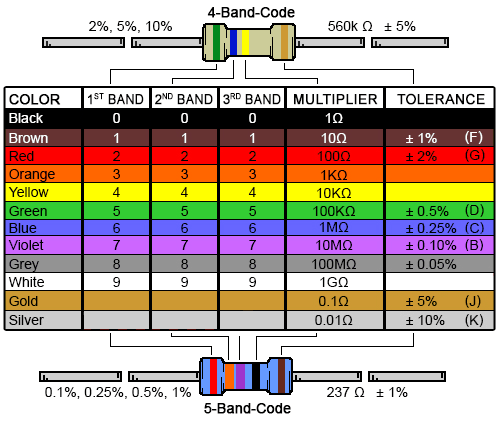
\includegraphics[width=0.8\linewidth]{img/resistor.png}  %[width=0.5\linewidth] ancho de la imagen respecto al ancho del texto --- {img/voz_humana.png} path completo de la imagen, en este caso, dentro de la carpeta "img"
    \caption{Tabla de colores de banda de resistores comerciales}    %texto que acompaña a la imagen por debajo
    \label{fig:tablaResistor}  %etiqueta para referenciar la figura
\end{figure}

\newpage

\subsection{Diagrama y esquemático del circuito}
La experiencia se realizó conectando el resistor otorgado a una fuente de alimentación y midiendo a través de la propia fuente los resultados de corriente que se leian una vez que se otorga valores de tensión predeterminados, empezando desde $0V$ subiendo por $0.2V$, $0.5V$, $1V$ y así sucesivamente sin un limite predeterminado.

Asimismo por la falta de limite de tensión la cual iba a ser sometida este resistor se veló por exponerla lo minimo posible a valores de potencia los cuales el mismo no admite, unicamente cerrando el circuito lo suficiente para tomar la medición y luego abriendo el circuito.


\begin{figure}[H]
    \centering  %figura centrada en el texto
    \begin{minipage}{0.48\textwidth}
        \centering
        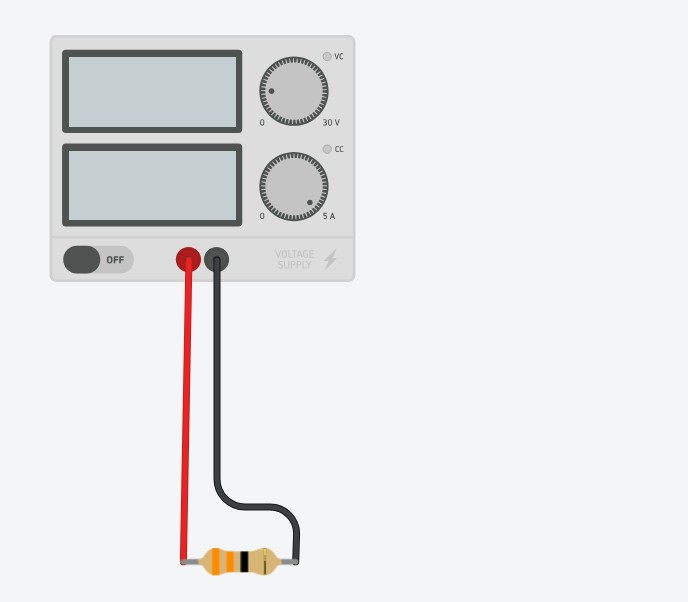
\includegraphics[width=1\linewidth]{img/diagrama.jpg}  %[width=0.5\linewidth] ancho de la imagen respecto al ancho del texto --- {img/voz_humana.png} path completo de la imagen, en este caso, dentro de la carpeta "img"
        \caption{Diagrama de conexión}    %texto que acompaña a la imagen por debajo
        \label{fig:diagrama1}  %etiqueta para referenciar la figura
    \end{minipage}
    \hfill
    \begin{minipage}{0.48\textwidth}
        \centering
        \begin{circuitikz}[american,scale=2,transform shape]
            \draw (0,0) to[V, invert, v=$V_1$] (0,3) -- (2,3)
            to[R, l=$R_1$] (2,0) -- (0,0);
        \end{circuitikz}
        \caption{Esquematico del circuito}
        \label{fig:esquematico1}
    \end{minipage}
\end{figure}
\newpage
\subsection{Resultados}
\begin{table}[htbp]
    \centering
    \begin{tabular}{|c|c|c|c|}
        \hline
        $V$ [V] & $\Delta V$ [V] & $I$ [A] & $\Delta I$ [A] \\
        \hline\hline
         0.0& 0.2000& 0.00& 0.005 \\
         0.2& 0.2004& 0.00& 0.005\\
         0.5& 0.2010& 0.01& 0.005\\
         1.0& 0.2020& 0.03& 0.005\\
         1.2& 0.05& 0.03& 0.005\\
         1.5& 0.05& 0.04& 0.005\\
         2.0& 0.05& 0.06& 0.005\\
         2.2& 0.05& 0.06& 0.005\\
         2.5& 0.05& 0.07& 0.005\\
         3.0& 0.05& 0.09& 0.005\\
         3.2& 0.05& 0.09& 0.005\\
         3.5& 0.05& 0.10& 0.005\\
         4.0& 0.05& 0.12& 0.005\\
         4.2& 0.05& 0.13& 0.005\\
         4.5& 0.05& 0.14& 0.005\\
         5.0& 0.05& 0.15& 0.005\\
         5.2& 0.05& 0.16& 0.005\\
         5.5& 0.05& 0.17& 0.005\\
         6.0& 0.05& 0.18& 0.005\\
         6.2& 0.05& 0.19& 0.005\\
         6.5& 0.05& 0.20& 0.005\\
         7.0& 0.05& 0.22& 0.005\\
         7.2& 0.05& 0.23& 0.005\\
         7.5& 0.05& 0.24& 0.005\\
         8.0& 0.05& 0.25& 0.005\\
         8.2& 0.05& 0.26& 0.005\\
         8.5& 0.05& 0.27& 0.005\\
         9.0& 0.05& 0.29& 0.005\\
         9.2& 0.05& 0.29& 0.005\\
         9.5& 0.05& 0.30& 0.005\\
         10.0& 0.05& 0.32& 0.005\\
         10.2& 0.05& 0.32& 0.005\\
         10.5& 0.05& 0.33& 0.005\\
         11.0& 0.05& 0.35& 0.005\\
         11.2& 0.05& 0.36& 0.005\\
         11.5& 0.05& 0.37& 0.005\\
         12.0& 0.05& 0.39& 0.005\\
         12.2& 0.05& 0.40& 0.005\\
         12.5& 0.05& 0.41& 0.005\\
         13.0& 0.05& 0.42& 0.005\\
         13.2& 0.05& 0.43& 0.005\\
         13.5& 0.05& 0.44& 0.005\\
        \hline
    \end{tabular}
    \caption{Mediciones de tension y corriente}
    \label{tab:mediciones1}
\end{table}
\begin{figure}[H]
    \begin{tikzpicture}
        \begin{axis}[
            title={Circuito 1},
            xlabel={Tensión [V]},
            ylabel={Corriente [A]},
            grid=major,
            width=13cm,
            height=13cm,
        ]

        % "only marks" draws just the points without connecting lines.
        % "error bars/.cd" enters the error bar configuration directory.
        \addplot+[
            color = blue,
            only marks,
            mark size=0.5pt,
            error bars/.cd,
            y dir=both, y explicit,
            x dir=both, x explicit
        ] table [x=x, y=y, x error=xerr, y error=yerr] {
            x   y   xerr yerr
            00.0   0.00  0.05  0.005
            00.2   0.00  0.05  0.005
            00.5   0.01  0.05  0.005
            01.0   0.03  0.05  0.005
            01.2   0.03  0.05  0.005
            01.5   0.04  0.05  0.005
            02.0   0.06  0.05  0.005
            02.2   0.06  0.05  0.005
            02.5   0.07  0.05  0.005
            03.0   0.09  0.05  0.005
            03.2   0.09  0.05  0.005
            03.5   0.10  0.05  0.005
            04.0   0.12  0.05  0.005
            04.2   0.13  0.05  0.005
            04.5   0.14  0.05  0.005
            05.0   0.15  0.05  0.005
            05.2   0.16  0.05  0.005
            05.5   0.17  0.05  0.005
            06.0   0.18  0.05  0.005
            06.2   0.19  0.05  0.005
            06.5   0.20  0.05  0.005
            07.0   0.22  0.05  0.005
            07.2   0.23  0.05  0.005
            07.5   0.24  0.05  0.005
            08.0   0.25  0.05  0.005
            08.2   0.26  0.05  0.005
            08.5   0.27  0.05  0.005
            09.0   0.29  0.05  0.005
            09.2   0.29  0.05  0.005
            09.5   0.30  0.05  0.005
            10.0   0.32  0.05  0.005
            10.2   0.32  0.05  0.005
            10.5   0.33  0.05  0.005
            11.0   0.35  0.05  0.005
            11.2   0.36  0.05  0.005
            11.5   0.37  0.05  0.005
            12.0   0.39  0.05  0.005
            12.2   0.40  0.05  0.005
            12.5   0.41  0.05  0.005
            13.0   0.42  0.05  0.005
            13.2   0.43  0.05  0.005
            13.5   0.44  0.05  0.005
        };

        \end{axis}
    \end{tikzpicture}
    \caption{Medición de corriente en relación a la tensión en el resistor}
    \label{fig:grafico1}
\end{figure}
\newpage
\section{Analisis de la experiencia 1}
\subsection{Observaciones}
Debido a exponer el resistor lo minimo posible a potencias las cuales no admite, el grafico se acerca en todo el rango de las mediciones a una recta directamente proporcional entre la tension y la corriente,
un comportamiento que resulta sencillo de modelar dentro del rango medido.

A pesar de que el resistor haya mantenido la mayoria de sus propiedades hasta el final de la medición
el mismo se calentó hasta quemarse y derretir la pintura que lo recubría, además de observarse humo saliendo del componente mientras el circuito se encontraba cerrado.

Se pudo ver en la experiencia el funcionamiento del resistor como limitador de corriente.
\section{Medición indirecta}
\subsection{Modelo a utilizar e incertidumbre}
El modelo a utilizar para verificar el valor del resistor es la Ley de Ohm.
\begin{align}
    V=I \cdot R
\end{align}
Como hemos medido tanto la tensión $V$ como la corriente $I$, despejamos la resistencia $R$
\begin{align}
    \frac{V}{I}=R
\end{align}
\subsubsection{Incertidumbre}
Debido a que estamos midiendo parametros físicos a través de una medición indirecta, hemos de propagar la incertidumbre a través de la ecuación dada.
\begin{align}
    \Delta R = \sqrt{(\frac{1}{I}\cdot \Delta V)^2+(\frac{-V}{I^2}\cdot \Delta I)^2}
\end{align}
\begin{table}[htbp]
    \centering
    \begin{tabular}{|c|c|c|c|}
        \hline
        $V$ [V] & $I$ [A] & $R_1$ [$\Omega$] & $\Delta R_1$ [$\Omega$] \\
        \hline\hline
         0.0& 0.00& -& - \\
         0.2& 0.00& -& -\\
         0.5& 0.01& 50.000& 25.495\\
         1.0& 0.03& 33.333& 5.800\\
         1.2& 0.03& 40.000& 6.872\\
         1.5& 0.04& 37.500& 4.851\\
         2.0& 0.06& 33.333& 2.900\\
         2.2& 0.06& 36.667& 3.167\\
         2.5& 0.07& 35.714& 2.649\\
         3.0& 0.09& 33.333& 1.933\\
         3.2& 0.09& 35.556& 2.052\\
         3.5& 0.10& 35.000& 1.820\\
         4.0& 0.12& 33.333& 1.450\\
         4.2& 0.13& 32.308& 1.301\\
         4.5& 0.14& 32.143& 1.202\\
         5.0& 0.15& 33.333& 1.160\\
         5.2& 0.16& 32.500& 1.063\\
         5.5& 0.17& 32.353& 0.996\\
         6.0& 0.18& 33.333& 0.967\\
         6.2& 0.19& 32.632& 0.898\\
         6.5& 0.20& 32.500& 0.850\\
         7.0& 0.22& 31.818& 0.758\\
         7.2& 0.23& 31.304& 0.714\\
         7.5& 0.24& 31.250& 0.684\\
         8.0& 0.25& 32.000& 0.671\\
         8.2& 0.26& 31.538& 0.636\\
         8.5& 0.27& 31.482& 0.612\\
         9.0& 0.29& 31.035& 0.562\\
         9.2& 0.29& 31.724& 0.574\\
         9.5& 0.30& 31.667& 0.554\\
         10.0& 0.32& 31.250& 0.513\\
         10.2& 0.32& 31.875& 0.522\\
         10.5& 0.33& 31.818& 0.505\\
         11.0& 0.35& 31.429& 0.471\\
         11.2& 0.36& 31.111& 0.454\\
         11.5& 0.37& 31.081& 0.441\\
         12.0& 0.39& 30.769& 0.415\\
         12.2& 0.40& 30.500& 0.401\\
         12.5& 0.41& 30.488& 0.391\\
         13.0& 0.42& 30.952& 0.387\\
         13.2& 0.43& 30.698& 0.375\\
         13.5& 0.44& 30.682& 0.367\\
        \hline
    \end{tabular}
    \caption{Medicion indirecta de resistencia}
    \label{tab:mediciones2}
\end{table}
\newpage
 A pesar de que conforme el valor de tensión aumenta, la incertidumbre se reduce hay que tomar en cuenta que el resistor que estamos midiendo permite una potencia maxima de $\frac{1}{4}W$, que siguiendo las cuentas:
 \begin{align}
    W &= V \cdot I\\
    W &= V \cdot \frac{V}{R}\\
    W &= \frac{V^2}{R}\\
    \frac{1}{4}W &= \frac{V^2}{33\Omega}\\
    \sqrt{\frac{33}{4}} &= V \approx 2.872V_{max}\\
 \end{align}
 La tensión maxima que admite ininterrumpidamente es de alrededor de 2.87V, lo cual significa que conforme se aumenta el valor de tensión también se arriesga quemar el resistor, y consecuentemente cambiar el valor de su resistencia.

 A pesar de ello elegí el valor de $13.5V$ y $0.44A$ debido a que tiene la menor incertidumbre dentro del rango medido.

\begin{tikzpicture}
\begin{axis}[
    title={Incertidumbres},
    xlabel={Resistencia[$R$]},
    % Set up the Y-axis for categories rather than continuous numbers
    ytick={1, 2},
    yticklabels={Fabricante, Medición ($13.5V$)},
    ymin=0, ymax=3, % Add padding above and below the categories
    xmin=30, xmax=35,
    grid=major, % Adds grid lines for easier reading
    width=10cm,
    height=5cm,
]

% Range 1: Group A (from 15 to 45)
% mark=* adds a solid circle at the start and end points
\addplot[color=blue, thick, mark=|] coordinates {(34.65, 1)(33,1) (31.35, 1)};

% Range 2: Group B (from 35 to 80)
% mark=| adds vertical ticks at the ends instead of circles
\addplot[color=red, thick, mark=|] coordinates {(30.315, 2)(30.682, 2) (31.049, 2)};


\end{axis}
\end{tikzpicture}
\subsection{Interpretación del gráfico}
Como se ve en el gráfico, la medición indirecta no coincide con los valores admitidos por el fabricante al momento de haber medido la última medición.
Esto puede ser debido a que este resistor estaba al $470\%$ de su potencia máxima y el valor de resistencia fue suficientemente comprometida para que no se encuentre en su rango de fabrica, pero no lo suficiente para que pese en el grafico \ref{fig:grafico1}.

Usando una medición previa se encontrará dentro del rango, ya que el resistor todavía no se quemó lo suficiente para variar la resistencia fuera del rango.

\begin{tikzpicture}
\begin{axis}[
    title={Incertidumbres},
    xlabel={Resistencia[$R$]},
    % Set up the Y-axis for categories rather than continuous numbers
    ytick={1, 2},
    yticklabels={Fabricante, Medición ($6.5V$)},
    ymin=0, ymax=3, % Add padding above and below the categories
    xmin=31, xmax=35,
    grid=major, % Adds grid lines for easier reading
    width=10cm,
    height=5cm,
]

% Range 1: Group A (from 15 to 45)
% mark=* adds a solid circle at the start and end points
\addplot[color=blue, thick, mark=|] coordinates {(34.65, 1)(33,1) (31.35, 1)};

% Range 2: Group B (from 35 to 80)
% mark=| adds vertical ticks at the ends instead of circles
\addplot[color=red, thick, mark=|] coordinates {(31.65, 2)(32.5, 2) (33.35, 2)};


\end{axis}
\end{tikzpicture}

En conclusión, si se ha de usar la medición indirecta a través de este método sería recomendable utilizar un resistor que admita la suficiente potencia para la totalidad del rango de valores a medir, para que el valor de la resistencia del mismo no varíe durante el tiempo.
\newpage
\section{Experiencia 2}
Se realizó un circuito serie con dos resistores y se midió la tensión en cada uno.

El instrumento utilizado para medir fue un multimetro ProsKit MT 1707.

\begin{figure}[H]
    \centering  %figura centrada en el texto
    \begin{minipage}{0.48\textwidth}
        \centering
        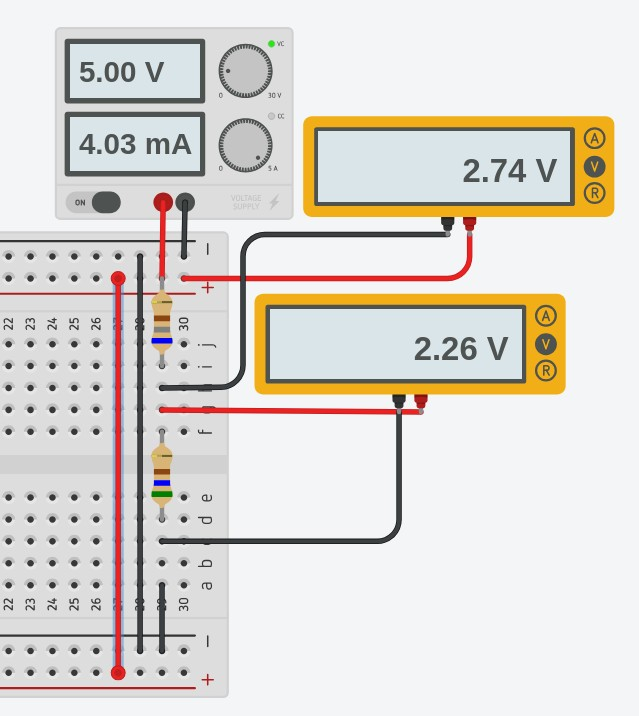
\includegraphics[width=1\linewidth]{img/diagrama2.jpg}  %[width=0.5\linewidth] ancho de la imagen respecto al ancho del texto --- {img/voz_humana.png} path completo de la imagen, en este caso, dentro de la carpeta "img"
        \caption{Diagrama de conexión}    %texto que acompaña a la imagen por debajo
        \label{fig:diagrama2}  %etiqueta para referenciar la figura
    \end{minipage}
    \hfill
    \begin{minipage}{0.48\textwidth}
        \begin{circuitikz}[american,scale=2,transform shape]
            \draw (0,3)
            % Voltage source on the top branch, going right
            to[V,invert, v=$V_s$] (3,3) 
            
            % First resistor on the right branch, going down
            to[R, l=$R_1$] (3,1.5) 
            
            % Second resistor continuing on the right branch, going down
            to[R, l=$R_2$] (3,0) 
            
            % Wire on the bottom branch, going left
            to[short] (0,0) 
            
            % Wire on the left branch, going up back to the source
            to[short] (0,3);
        \end{circuitikz}
        \centering
        \caption{Esquematico del circuito}
        \label{fig:esquematico2}
    \end{minipage}
\end{figure}

\begin{table}[htbp]
    \centering
    \begin{tabular}{|c|c|c|c|}
        \hline
        $V_{R_1}$ [V] & $V_{R_2}$ [V] & $\Delta V{R_1}$ [V] & $\Delta V_{R_2} [V]$\\
        \hline\hline
         2.76&2.24 &0.005 &0.005 \\
        \hline
    \end{tabular}
    \caption{Valores medidos en ambos resistores}
    \label{tab:mediciones3}
\end{table}

Siendo:
\begin{align}
    V_s &= 5V\\
    R_1 &= 680 \Omega\\
    R_2 &= 560 \Omega\\
\end{align}
\subsection{Ley de Kirchoff de tensiones}
Según la ley de Kirchoff la suma de las tensiones de una rama es igual a cero.
Haciendo ley de Kirchoff en el circuito dado:
\begin{align}
    V_s = V_{R_1} + V_{R_2}\\
    V_s = R_1 \cdot I + R_1 \cdot I\\
    V_s = I(R_1+R_2)\\
    5V = I( 680 \Omega + 560 \Omega)\\
    \frac{5V}{1240 \Omega} = I \\
    4,03mA \approx I\\
\end{align}
Con la corriente podemos determinar la caida de tensión en ambos resistores
\begin{align}
    V_{R_1} = 680 \Omega \cdot \frac{5V}{1240 \Omega}\\
    V_{R_2} = 560 \Omega \cdot \frac{5V}{1240 \Omega}\\
    V_{R_1} \approx 2.74V\\
    V_{R_2} \approx 2.26V\\
    V_{R_1} + V_{R_2} = 5V 
\end{align}

Lo cual se verifica con las mediciones. La ley de Kirchoff se cumple.
\section{Mismo circuito, diferentes valores de Resistencia}
Se realizó exactamente el mismo circuito, pero cambiando el valor de $R_1$ y $R_2$ a $1M\Omega$ en ambos casos.

Haciendo ley de Kirchoff en el circuito dado:
\begin{align}
    V_s = V_{R_1} + V_{R_2}\\
    V_s = R_1 \cdot I + R_1 \cdot I\\
    V_s = I(R_1+R_2)\\
    5V = I(2M\Omega)\\
    \frac{5V}{2M\Omega} = I \\
    2.5\mu A = I\\
\end{align}
Con la corriente podemos determinar la caida de tensión en ambos resistores
\begin{align}
    V_{R_1} = 1 M\Omega \cdot \frac{5V}{1 M\Omega}\\
    V_{R_2} = 1 M\Omega \cdot \frac{5V}{1 M\Omega}\\
    V_{R_1} = 2.5V\\
    V_{R_2} = 2.5V\\
    V_{R_1} + V_{R_2} = 5V 
\end{align}
Pero estos valores no cumplen con las mediciones:
\begin{table}[htbp]
    \centering
    \begin{tabular}{|c|c|c|c|}
        \hline
        $V_{R_1}$ [V] & $V_{R_2}$ [V] & $\Delta V_{R_1}$ [V] & $\Delta V_{R_2} [V]$\\
        \hline\hline
         2.40&2.37 &0.005 &0.005 \\
        \hline
    \end{tabular}
    \caption{Valores medidos en ambos resistores}
    \label{tab:mediciones4}
\end{table}

La impedancia del multimetro utilizado es de $10M\Omega$, lo cual para circuitos de baja resitencia no influye mucho en la medicion, pero en el caso de este circuito el mismo afecta a la medicion y crea una nueva corriente al estar en paralelo, llevando a que las mediciones no cumplan la ley de tension de Kirchoff, ya que el circuito diagramado no es el mismo cuando se mide, ya que afecta el voltimetro.

\section*{Circuito al medir $R_1$}

\begin{circuitikz}[american,scale=2,transform shape]
  % Main loop (same as before)
  \draw (0,3)
    to[V,invert, v=$V_s$] (3,3) 
    to[R, l=$R_1$] (3,1.5) 
    to[R, l=$R_2$] (3,0) 
    to[short] (0,0) 
    to[short] (0,3);

  % Branch parallel to R1
  \draw (3,3) 
    to[short, *-] (5,3)         % Wire goes right (starts with a dot)
    to[R, l=$R_{Voltimetro}$] (5,1.5)      % Resistor going down
    to[short, -*] (3,1.5);      % Wire goes left back to main branch (ends with a dot)
\end{circuitikz}

\vspace{1cm} % Adds space between the two circuits

\section*{Circuito al medir $R_2$}

\begin{circuitikz}[american,scale=2,transform shape]
  % Main loop
  \draw (0,3)
    to[V,invert, v=$V_s$] (3,3) 
    to[R, l=$R_1$] (3,1.5) 
    to[R, l=$R_2$] (3,0) 
    to[short] (0,0) 
    to[short] (0,3);

  % Branch parallel to R2
  \draw (3,1.5) 
    to[short, *-] (5,1.5)       % Wire goes right (starts with a dot)
    to[R, l=$R_{Voltimetro}$] (5,0)        % Resistor going down
    to[short, -*] (3,0);        % Wire goes left back to main branch (ends with a dot)
\end{circuitikz}

Planteandolo de esta manera:
\begin{align}
    R_{eq} = \frac{1}{\frac{1}{1M\Omega}+\frac{1}{10M\Omega}}+1M\Omega\\
    R_{eq} = \frac{1}{\frac{11}{10M\Omega}}+1M\Omega\\
    R_{eq} = \frac{10M\Omega}{11}+1M\Omega\\
    R_{eq} = \frac{21M\Omega}{11}\\
    I_{Total} = \frac{5V}{\frac{21M\Omega}{11}}\\ 
    I_{Total} \approx 2.62\mu A  
\end{align}
Ahora calculo $V_{R_2}$ y con eso saco la corriente que carga el voltimetro
\begin{align}
    V_{R_2} = I_{Total}\cdot R_2\\
    V_{R_2} \approx 2.619V \\
    V_{R_{Voltimetro}} = V{R_1} = V_s - V_{R_2} \\
    V_{R_{Voltimetro}} = V{R_1} \approx 5V - 2.619V \\
    V_{R_{Voltimetro}} = V{R_1} \approx 2.381V  \\
    I_{R_{Voltimetro}} = \frac{V{R_{Voltimetro}}}{10M\Omega}\\
    I_{R_{Voltimetro}} \approx \frac{2.381V}{10M\Omega}\\
    I_{R_{Voltimetro}} \approx 0.2381 \mu A 
\end{align}
Como se ve, la corriente del circuito al medir no es la misma que el circuito original sin medir, por ende al medir tension afectamos la medicion y debido a ello surge este problema.

En estos casos, al ser el comportamiento de los circuitos exactamente el mismo seria analogo medir en un circuito donde la impedancia sea irrisoriamente alta, como el primero, donde casi no afecta.  Mientras que la relacion entre los resistores sea el mismo, la caida de tensión sera la misma (en identicos $\frac{V_s}{2}$ en cada resistor), pudiendo confirmar con Kirchoff.
\newpage
\section{Simulacion en LTSpice}
\begin{figure}[H]
    \centering
    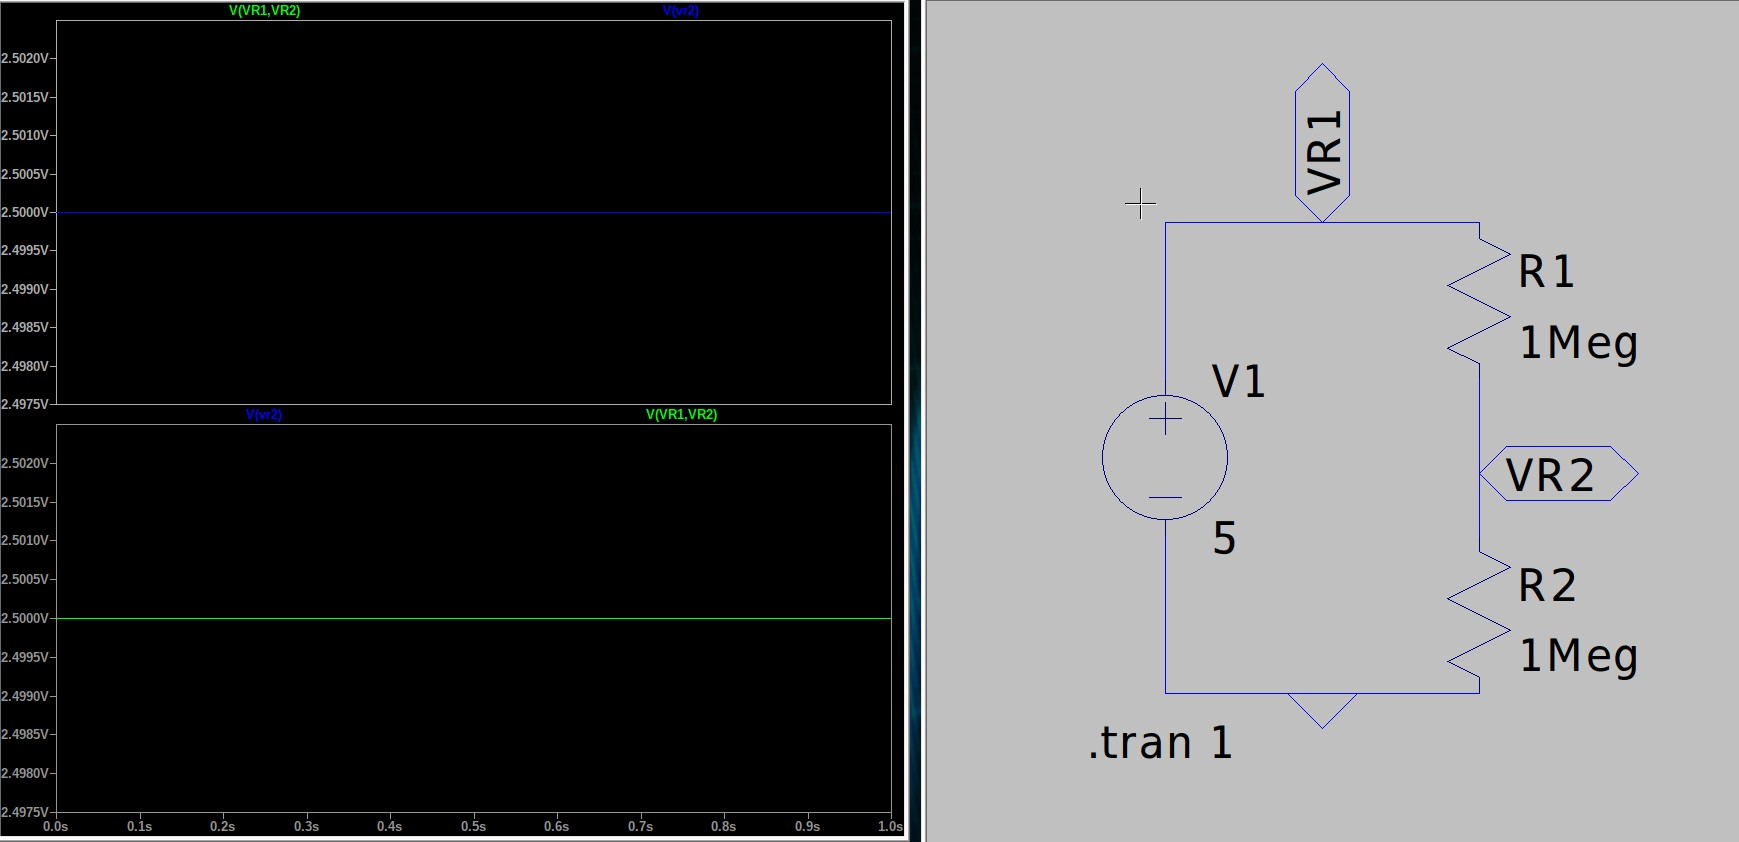
\includegraphics[width=0.8\linewidth]{img/simulacion1.jpg}  %[width=0.5\linewidth] ancho de la imagen respecto al ancho del texto --- {img/voz_humana.png} path completo de la imagen, en este caso, dentro de la carpeta "img"
    \caption{Simulacion}    %texto que acompaña a la imagen por debajo
    \label{fig:simulacion1}  %etiqueta para referenciar la figura
\end{figure}
Al ser LTSpice un simulador, utiliza modelos fisicos para simular los circuitos, y por ende no debe de "poner el voltimetro" para medir, sino simplemente mostrar el valor de tensión en ese punto. Debido a que los valores de tensión medidos no son los mismos que los calculados por el efecto de carga del multimetro, y no un fallo en los calculos que de exactamente lo mismo que lo calculado es coherente, y es aproximadamente lo que pasa en el circuito, siendo mas cercano que lo medido.

\subsection{IA para simular}
Se utilizó Gemini con una captura del esquematico e instrucciones para realizar un archivo .asc que simule el mismo en LTSpice con 2 resistencias de $1M\Omega$ y una fuente de $5V$.

El resultado a pesar de ser alentador no fue funcional, siendo imposible simular sin modificarlo.

\begin{figure}[H]
    \centering
    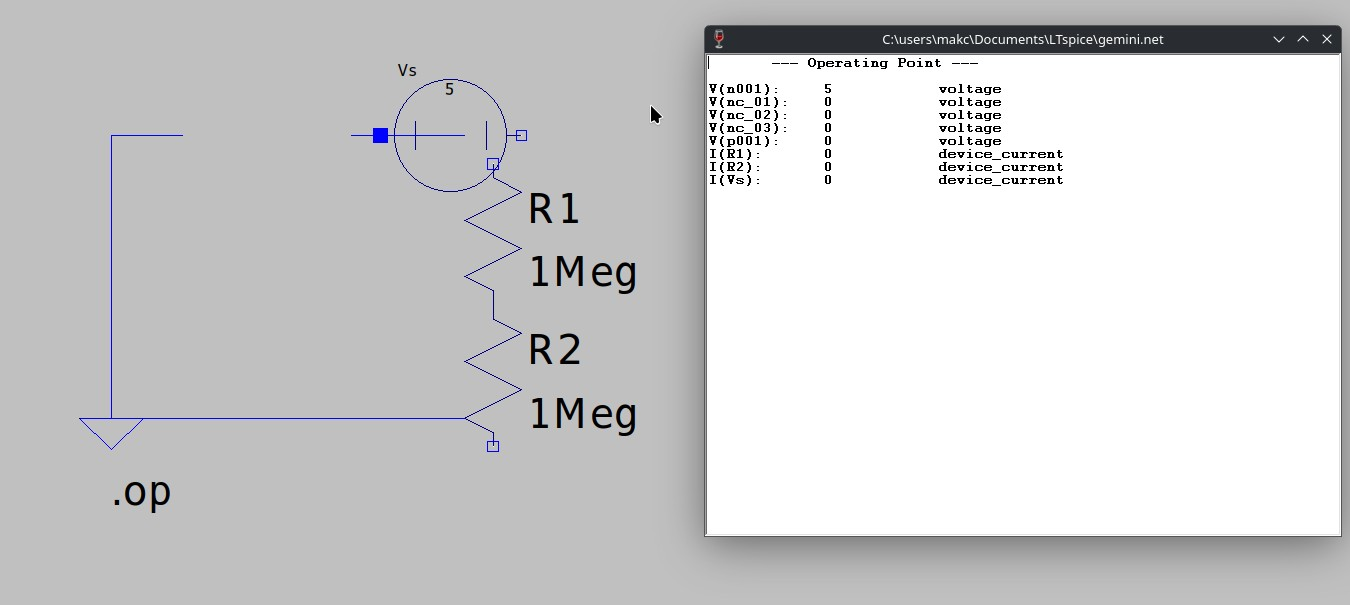
\includegraphics[width=0.8\linewidth]{img/simulaciongemini.jpg}  %[width=0.5\linewidth] ancho de la imagen respecto al ancho del texto --- {img/voz_humana.png} path completo de la imagen, en este caso, dentro de la carpeta "img"
    \caption{Simulacion construida por Gemini}    %texto que acompaña a la imagen por debajo
    \label{fig:gemini1}  %etiqueta para referenciar la figura
\end{figure}
\begin{figure}[H]
    \centering
    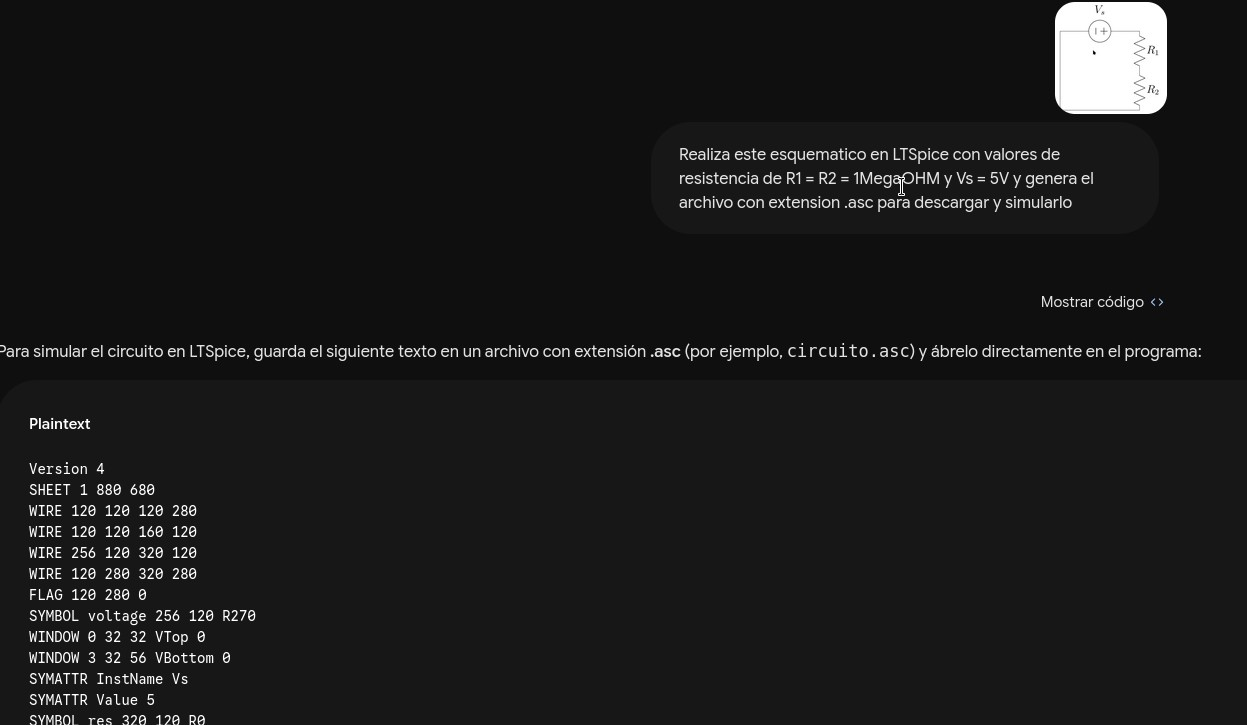
\includegraphics[width=0.8\linewidth]{img/gemini.jpg}  %[width=0.5\linewidth] ancho de la imagen respecto al ancho del texto --- {img/voz_humana.png} path completo de la imagen, en este caso, dentro de la carpeta "img"
    \caption{Prompt otorgado}    %texto que acompaña a la imagen por debajo
    \label{fig:gemini2}  %etiqueta para referenciar la figura
\end{figure}

\section{Conclusiones}
Las dos experiencias realizadas fueron pertinentes no sólo para familiarizarse con métodos de resolución de circuitos y componentes elementales, sino también para entender la brecha entre la teoría y la práctica, y como lidiar con la imprecisión e incertidumbre propia al trabajar con magnitudes físicas.

\end{document}